\documentclass[border=2pt]{standalone}
\usepackage{pgfplots}
\pgfplotsset{compat=1.18}
\begin{document}
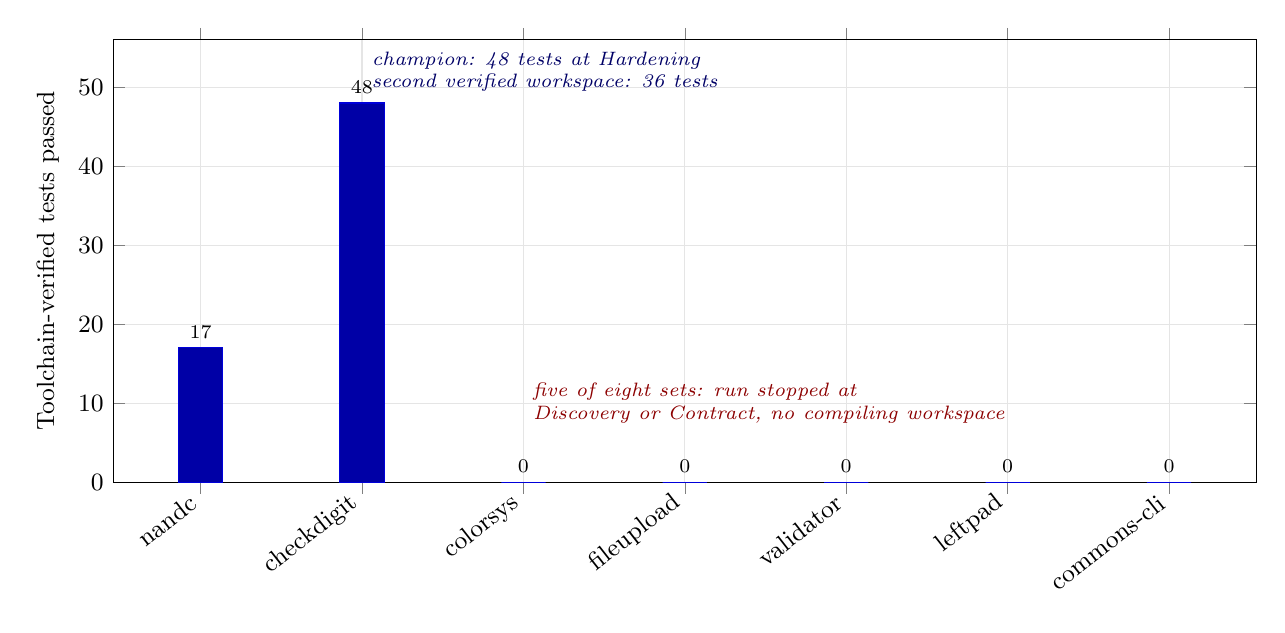
\begin{tikzpicture}
\begin{axis}[
  x=2.05cm,
  width=15.5cm,
  height=7.2cm,
  ylabel={Toolchain-verified tests passed},
  ymin=0, ymax=56,
  symbolic x coords={nandc,checkdigit,colorsys,fileupload,validator,leftpad,commons-cli},
  xtick=data,
  x tick label style={rotate=38, anchor=east, font=\small},
  ybar=3pt,
  bar width=16pt,
  grid=major,
  grid style={gray!20},
  tick label style={font=\small},
  label style={font=\small},
  enlarge x limits=0.09,
  nodes near coords,
  every node near coord/.append style={font=\scriptsize},
  clip=false,
]
% Final campaign record (.artifacts/experiments/SUMMARY.md): best
% toolchain-verified test counts per problem set. nandc champion lineage
% peaked at 17 (c3-h3); checkdigit peaked at 48 (c10b) with a second
% verified workspace at 36 (c11b). Every other set ended with no
% compiling workspace, so its bar sits at height 0 with the run stopped
% at Discovery or Contract.
\addplot[fill=blue!65!black, draw=blue!85!black] coordinates {
  (nandc,17) (checkdigit,48) (colorsys,0) (fileupload,0)
  (validator,0) (leftpad,0) (commons-cli,0)
};
\node[font=\scriptsize\itshape, text=blue!40!black, align=left, anchor=west]
  at (axis cs:checkdigit,52) {champion: 48 tests at Hardening\\second verified workspace: 36 tests};
\node[font=\scriptsize\itshape, text=red!55!black, align=left, anchor=west]
  at (axis cs:colorsys,10) {five of eight sets: run stopped at\\Discovery or Contract, no compiling workspace};
\end{axis}
\end{tikzpicture}
\end{document}
